\documentclass[11pt]{article}
% Shared preamble of the RMC kernel write-ups (% Shared preamble of the RMC kernel write-ups (% Shared preamble of the RMC kernel write-ups (\input{preamble} after \documentclass).
\usepackage[margin=1in]{geometry}
\usepackage{amsmath,amssymb,bm}
\usepackage{graphicx}
\usepackage{booktabs}
\usepackage{hyperref}

\newcommand{\dd}{\,\mathrm{d}}
\newcommand{\Ein}{E}
\newcommand{\Eout}{E'}
\newcommand{\Ecm}{E_{c}}
\newcommand{\mucm}{\mu_{c}}
\newcommand{\mulab}{\mu_0}

% Common closing section: how the verification figures are produced
\newcommand{\verificationmethod}{%
Each figure is produced by \texttt{verification/verify\_laws.py}. For an incident
energy $\Ein$ along $+z$, $10^6$ collisions are sampled with MC/DC's own reaction
sampler (\texttt{sample\_elastic\_scattering}, \texttt{sample\_inelastic\_scattering}
or \texttt{sample\_fission}), and every emitted neutron is histogrammed in
$48 \times 24$ bins of $(\Eout, \mulab)$, with $\mulab$ the lab cosine to $+z$. The
inverted kernel used by RMC is integrated over the same bins (Gauss--Legendre panels;
two-body lines are split where $\mulab^*(\Eout)$ crosses a cosine edge), multiplied by
the number of collisions, and compared with a $\chi^2$ test over bins with at least 5
expected counts (the rest pooled into one bin). The tables list $\chi^2/\mathrm{dof}$,
its $p$-value, the emitted neutrons per collision (sampled vs.\ the integral of the
inverted kernel), and the largest relative change of a bin integral when the
quadrature panels are doubled. Left panels: outgoing-energy marginal; middle:
lab-cosine marginal; right: per-bin $z = (\text{sampled} - \text{inverted}) /
\sqrt{\text{inverted}}$.}
 after \documentclass).
\usepackage[margin=1in]{geometry}
\usepackage{amsmath,amssymb,bm}
\usepackage{graphicx}
\usepackage{booktabs}
\usepackage{hyperref}

\newcommand{\dd}{\,\mathrm{d}}
\newcommand{\Ein}{E}
\newcommand{\Eout}{E'}
\newcommand{\Ecm}{E_{c}}
\newcommand{\mucm}{\mu_{c}}
\newcommand{\mulab}{\mu_0}

% Common closing section: how the verification figures are produced
\newcommand{\verificationmethod}{%
Each figure is produced by \texttt{verification/verify\_laws.py}. For an incident
energy $\Ein$ along $+z$, $10^6$ collisions are sampled with MC/DC's own reaction
sampler (\texttt{sample\_elastic\_scattering}, \texttt{sample\_inelastic\_scattering}
or \texttt{sample\_fission}), and every emitted neutron is histogrammed in
$48 \times 24$ bins of $(\Eout, \mulab)$, with $\mulab$ the lab cosine to $+z$. The
inverted kernel used by RMC is integrated over the same bins (Gauss--Legendre panels;
two-body lines are split where $\mulab^*(\Eout)$ crosses a cosine edge), multiplied by
the number of collisions, and compared with a $\chi^2$ test over bins with at least 5
expected counts (the rest pooled into one bin). The tables list $\chi^2/\mathrm{dof}$,
its $p$-value, the emitted neutrons per collision (sampled vs.\ the integral of the
inverted kernel), and the largest relative change of a bin integral when the
quadrature panels are doubled. Left panels: outgoing-energy marginal; middle:
lab-cosine marginal; right: per-bin $z = (\text{sampled} - \text{inverted}) /
\sqrt{\text{inverted}}$.}
 after \documentclass).
\usepackage[margin=1in]{geometry}
\usepackage{amsmath,amssymb,bm}
\usepackage{graphicx}
\usepackage{booktabs}
\usepackage{hyperref}

\newcommand{\dd}{\,\mathrm{d}}
\newcommand{\Ein}{E}
\newcommand{\Eout}{E'}
\newcommand{\Ecm}{E_{c}}
\newcommand{\mucm}{\mu_{c}}
\newcommand{\mulab}{\mu_0}

% Common closing section: how the verification figures are produced
\newcommand{\verificationmethod}{%
Each figure is produced by \texttt{verification/verify\_laws.py}. For an incident
energy $\Ein$ along $+z$, $10^6$ collisions are sampled with MC/DC's own reaction
sampler (\texttt{sample\_elastic\_scattering}, \texttt{sample\_inelastic\_scattering}
or \texttt{sample\_fission}), and every emitted neutron is histogrammed in
$48 \times 24$ bins of $(\Eout, \mulab)$, with $\mulab$ the lab cosine to $+z$. The
inverted kernel used by RMC is integrated over the same bins (Gauss--Legendre panels;
two-body lines are split where $\mulab^*(\Eout)$ crosses a cosine edge), multiplied by
the number of collisions, and compared with a $\chi^2$ test over bins with at least 5
expected counts (the rest pooled into one bin). The tables list $\chi^2/\mathrm{dof}$,
its $p$-value, the emitted neutrons per collision (sampled vs.\ the integral of the
inverted kernel), and the largest relative change of a bin integral when the
quadrature panels are doubled. Left panels: outgoing-energy marginal; middle:
lab-cosine marginal; right: per-bin $z = (\text{sampled} - \text{inverted}) /
\sqrt{\text{inverted}}$.}


\title{Inverted kernel: evaporation spectrum (ENDF Law 9)}
\date{}

\begin{document}
\maketitle

\noindent Code: \texttt{evaluate\_evaporation}, \texttt{evaporation\_normalization} in
\texttt{mcdc/rmc/evaluate.py}.

\section{What MC/DC samples}

\texttt{sample\_evaporation}: with the nuclear temperature $\theta(\Ein)$ (tabulated,
interpolated by \texttt{evaluate\_data} with the ENDF interpolation laws of the data;
none listed means linear-linear), restriction energy $U$, $L = \Ein - U$,
$w = L/\theta$ and $g = 1 - e^{-w}$,
\begin{equation}
  x = -\theta\ln\big[(1 - g\xi_1)(1 - g\xi_2)\big],\qquad \text{accepted if } 0 \le x \le L .
\end{equation}

\section{Density of the sampled value}

Each term $Y_j = -\theta\ln(1 - g\xi_j)$ is an exponential with mean $\theta$
truncated to $[0, L]$: $P(Y_j \le y) = (1 - e^{-y/\theta})/g$, density
$e^{-y/\theta}/(\theta g)$ on $[0, L]$. For $0 \le x \le L$ the density of the sum is
the convolution
\begin{equation}
  \int_0^{x}\frac{e^{-y/\theta}}{\theta g}\,\frac{e^{-(x-y)/\theta}}{\theta g}\dd y
  = \frac{x\,e^{-x/\theta}}{\theta^2 g^2} ,
\end{equation}
(sums above $L$ are rejected), so the accepted value has the Law 9 density
\begin{equation}
  p(x \mid \Ein) = \frac{x\,e^{-x/\theta}}{\theta^2 I(w)},\qquad
  I(w) = \int_0^w s e^{-s}\dd s = 1 - e^{-w}(1 + w),\qquad 0 \le x \le \Ein - U .
\end{equation}
For $w < 10^{-3}$, $I(w) = w^2\left(\tfrac12 - \tfrac w3 + \tfrac{w^2}{8} -
\tfrac{w^3}{30}\right)$ avoids cancellation. The support is $[0, \Ein - U]$ (empty below
$U$); the density is smooth on it, so its end points are the only breakpoints.

\section{Reaction kernel}

The data used here (C-12 MT-28, MT-91) are in the lab frame with isotropic angles:
$f_L(\Eout, \mulab \mid \Ein) = Y\,p(\Eout \mid \Ein)/2$. In the COM frame the product
is $f_C$ and $f_L = f_C\sqrt{\Eout/\Ecm}$.

\paragraph{Data loading fix.} C-12's evaporation temperature tables have no
interpolation regions (ACE $NR = 0$, meaning linear-linear). The generator wrote empty
interpolation arrays, which MC/DC's \texttt{DataTable} rejected, so C-12 could not be
loaded at all; \texttt{fix/evaporation-maxwellian-loading} defaults them to
linear-linear.

\section{Verification}
\verificationmethod

\begin{center}
\begin{tabular}{rrrrrrr}
\toprule
$E$ [eV] & samples & bins & $\chi^2/\mathrm{dof}$ & $p$ & yield (sampled / inverted) & quad. err. \\
\midrule
1.2e+07 & 1e+06 & 841 & 813.7/841 & 0.744 & 1.00000 / 1.00000 & 1.7e-14 \\
1.8e+07 & 1e+06 & 697 & 642.5/697 & 0.931 & 1.00000 / 1.00000 & 2.3e-14 \\
\bottomrule
\end{tabular}

\end{center}

\begin{figure}[h]
  \centering
  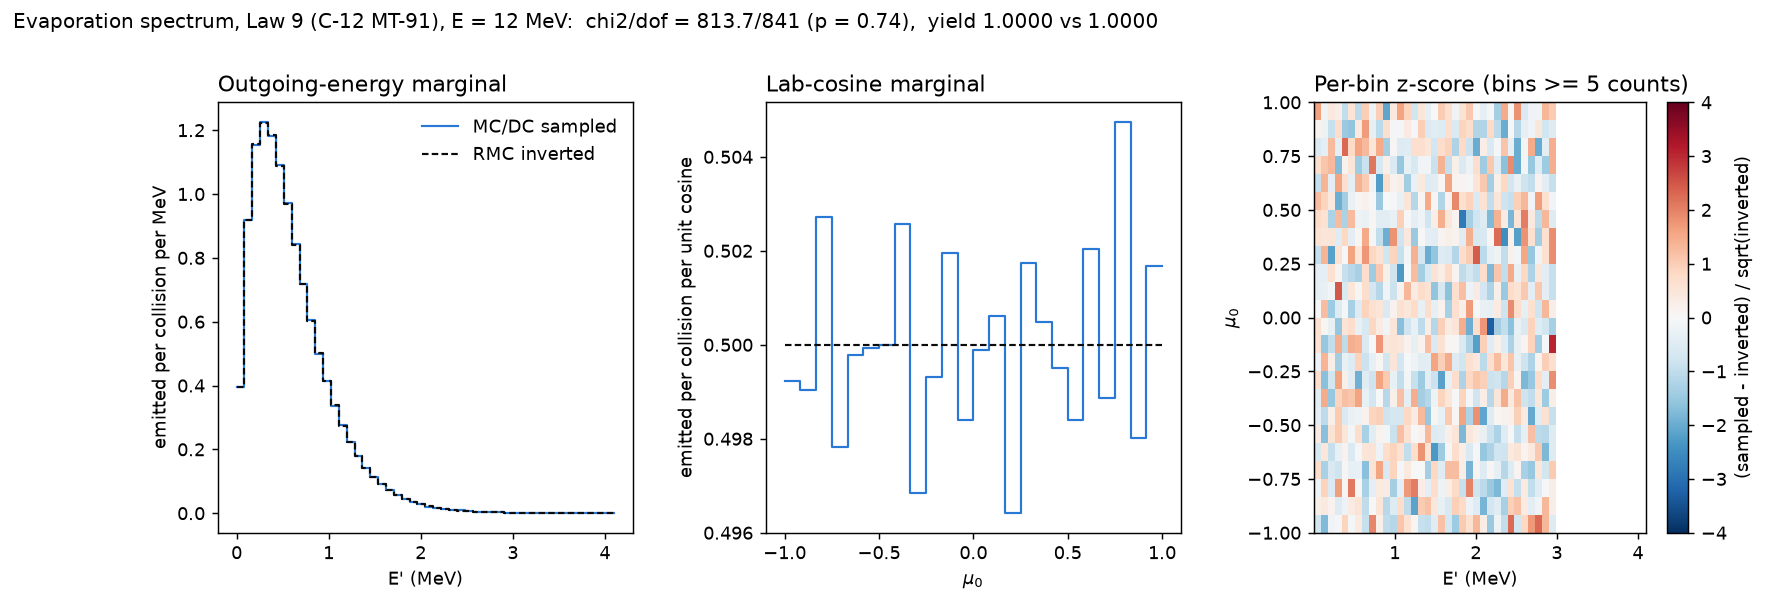
\includegraphics[width=\textwidth]{figures/evaporation/evaporation_E1p2e07.png}
  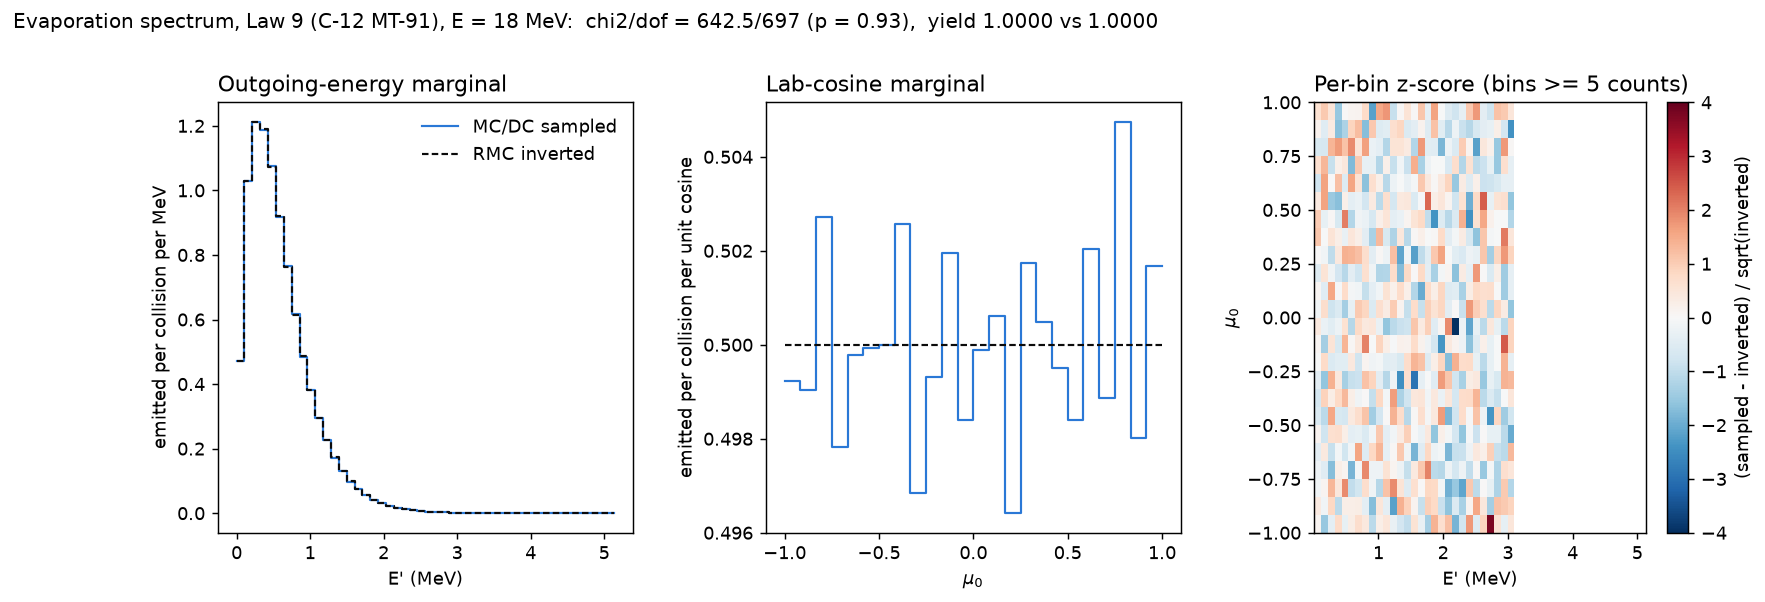
\includegraphics[width=\textwidth]{figures/evaporation/evaporation_E1p8e07.png}
  \caption{C-12 MT-91 (continuum inelastic, evaporation spectrum with
  $\theta = 0.3$\,MeV, $U = 7.89$\,MeV, lab frame, isotropic) at 12 and 18\,MeV.}
\end{figure}

\end{document}
